\chapter{Background} \label{Background}

In this chapter we will discuss concepts and technologies used to develop our system.

\section{Non-Volatile Memory and Persistent Memory}
    
    %\tk{NVM - briefly what it is, and what is it good for; a paragraph about the history of NVM -- where did it come from, how it evolved, what is the current status (e.g. one can buy some hardware but it is still relatively slow and expensive, drivers are available; what are the most popular technologies within the NVM-world?; is NVM the same as PM?}
    
    \subsection{Definitions}
    \tk{This might be misleading. Let's call NVM only the new technology, not just any computer storage.}
        \NVM (NVM) is a class of memory storage devices which are able to keep data after power outage. Consequently, they are suitable for systems which rely on data durability, such as database systems.
        In fact, NVM is one of the crucial components of most computers, as the most popular data storages: HDD and SSD drives are part of NVM family.
        A noticable drawback of this type of memory is a fact that it is much slower than their volatile counterparts. 
        Currently high-performance NVM solution is expensive and offers low capacity while still having a significant lack of performance in comparison to DRAM memory. 
        The performance of NVM, however, is still improving and the gap between NVM and DRAM is expected to be insignificant in the future. 
        
        \PM (PM) is a directly byte-addressable, non-volatile memory which can be accessed via the memory bus.
        
    \subsection{Access to NVM \cite{PmemAccess}}
        \tk{Correct me if I'm wrong, but it seems to me that at least Intel uses the same technology to created PM as well as for a new kind of SSDs, which are treated by the operating system as block devices (Intel Optane?).}
    
        In most computer applications access to data storage proceeds as follows:
        \begin{itemize}
            \item Application uses the file system API to access the files.
            \item File system performs read and write operations through a driver.
            \item All data transferred during those operations is composed of blocks, typically of size 4KB.
        \end{itemize}
        The solution described above is inadequate from the point of view of PM, because it makes programmers unable to utilize low latency byte-addressable direct access supported by the hardware.
        To solve this issue the support for \DAX (DAX) was incorporated into operating systems.
        In this approach persistent memory-aware file system is used to map virtual addresses to physical addresses in PM. 
        It allows applications to directly access individual bytes of the storage without the necessity to operate on entire blocks. The processes attach a region of mapped persistent memory to their address space and simply use it as an ordinary operating memory  segment.
      
    \subsection{Emulation}
        %\tk{What is emulation, what is it for? When it can be use, as opposed1 to what?}
        Persistent memory is not easily available and during this project we were not able to use it. 
        To examine its features in an application it is possible to emulate it by marking 
        using a file system with DAX support, by marking ordinary RAM segments as PM.\cite{PmemEmulation}
        % Alternatively, a regular shared memory segment can be used for emulation
        Emulation of the \PM is not obligatory during the development of the project, however, it is required to achieve a sufficient performance of the final product. 
        Emulation is based on DRAM memory, which is recognized by operating system as persistent memory region.
        \PM emulated in such way will not keep data after power outage, but it will provide performance comparable with hardware solution.
        %kn: what about the files which we use to emulate PM?
        
    \subsection{Developing applications for NVM}
        %\tk{Maybe something like: developing applications for NVM or NVM-enables applications?}
        
        \tk{This subsection requires more details. Why do we get corrupted or incomplete data? Why a mutex won't be released? Because after a crash, the state of processes/threads is not restored. Processes operate in RAM, cache and processor registers, the contents all of which can be lost event though NVM is used. }
    
        Programming for persistent memory differs from programming for volatile memory. 
        In case of this project there are two most important differences that should be considered.
        
        Firstly, persistent memory is not reinitialized after the application restart. 
        It implies that corrupted or incomplete data is kept in data structure and may cause incorrect functioning of the program or crashes. 
        To prevent such situations mechanism similar to ACID transactions offered by database management systems should be provided. \tk{NVM does not require ACID! only atomicity}
        It needs to guarantee:
        \label{ACID}
        \begin{itemize}
            \item Atomicity - Either all operations in transaction will be performed or none of them. 
            \item Consistency - If a system is consistent at the beginning of the transaction, it has to be consistent at the end of the transaction.
            \item Isolation - Changes made during the transaction will not be visible to other users until the transaction will be committed.
            \item Durability - Committed transactions cannot be recalled.
        \end{itemize}
        %\tk{Too concise. What transactions? What do they need to guarantee?}
        
        Second problem is a synchronisation mechanism. 
        Using mutexes in persistent memory may cause unintended behaviour. 
        If a thread crashes after locking a mutex, it may never unlock which results in a deadlock. 
      
\section{Persistent Memory Development Kit}

    \subsection{Overview}
        Persistent Memory Development Kit (PMDK) \cite{PmemIo} is a set of libraries developed by Intel Corporation, which aim is to support persistent memory programming. 
        It is based on memory-mapped files (POSIX \texttt{mmap} system call). 
        PMDK consists of 10 libraries suitable for various tasks, most important of which are described below. 
        It also includes examples which demonstrate how to use each of those libraries and their documentation. 
        Demonstration how to use those libraries will be shown in the next chapter.
        
    %    \tk{The mentioned librariees need not to be in separate subsections, just use enumeration. Also use \texttt{the proper font} for libraries' names. Add that you demonstrate how to use those libraries later on.}
    
    \begin{enumerate}
    
    \item
        \texttt{Libpmem} library provides a low-level persistent memory API for C language. 
        It requires developers to handle memory allocation and flush changes to persistent memory by themselves. 
        It also does not provide transactions.
        Other libraries included in PMDK are based on \texttt{libpmem} and call it internally.
    
    \item
        \texttt{Libpmemobj} is a high-level persistent memory library providing API for C language.
        In contrast to \texttt{libpmem} library, it has implementations of some high-level concepts: 
        \begin{itemize}
            \item Persistent memory management - persistent memory allocation mechanism and persistent memory pointers are provided.
            \item Transactions - memory snapshot is created and can be restored after failure of a transaction block.
            \item Concurrency support - API similar to pthread API allows to use mutexes which are automatically unlocked when a crash occurs.
            \item Data structures - non-transactional doubly-linked list similar to the one implemented in C standard library is provided. 
        \end{itemize}
        
    \item
        \texttt{Libpmemobj++} library provides a C++ bindings for \texttt{libpmemobj}.
        It allows to create object-oriented applications providing API similar to C++ Standard Template Library (STL), including smart pointers and mutexes compatible with STL locks (std::shared\_lock \cite{SharedLock}, std::unique\_lock \cite{UniqueLock}).
        Unfortunately it does not support polymorphism, so objects stored in persistent memory cannot use this mechanism.
    \end{enumerate}
\section{Distributed hash table} % distributed hash table

    This section covers the general concepts of creating a distributed system for the implemented data structure. 

    \subsection{Amazon Dynamo}
        As already mentioned in Chapter~\ref{Introduction}, the architecture of \DHTS follows the design principles of \Dynamo. 
        Since Amazon is one of the largest e-commerce companies, their services are used by millions of users concurrently.
        Worldwide range of services imply allocating servers and network components around the world.
        In such architecture single units failures are inevitable and have to be taken into account when creating the system.
        
        \Dynamo is highly available key-value storage system.
        It is used by some core services of Amazon to provide the "always-on" experience, for example Amazon Simple Storage Service \cite{AmazonS3} also known as Amazon S3.
        In Dynamo the key principles are:
        
        \begin{itemize}
            \item \textit{Incremental scalability}:
                The system should be able to scale out easily.
                Connecting a new node to the network cannot have a significant impact on the system performance.
            \item \textit{Symmetry}:
                Each node in the system is equal and has the same set of responsibilities as its peers. 
                There is no superior unit to control the system, so that its maintenance is simplified.
            \item \textit{Decentralisation}:
                This is an extension of the symmetry principle.
                A centralised control of the system could result in an outage and be a bottleneck of the whole network.
                Therefore, decentralised peer-to-peer techniques should be favoured during development.
                It can lead to better scalable system with higher availability.
            \item \textit{Heterogeneity}:
                The system should be implemented in a way that allows control of work distribution. 
                The amount of work given to a node should be proportional to its computing capabilities.
        \end{itemize}

    \subsection{Consistent hashing}
        As previously stated, the described system is composed of many nodes. 
        Their number varies constantly, since the nodes may join and leave the network at any time.
        This requires different approach when distributing the hashtable between the nodes.
        Traditional method causes nearly all keys to be remapped when a new node appears.
        This would significantly decrease our system performance since the various elements in the hash table would have to constantly migrate from one node to another.
        
        A provided solution is called \textit{consistent hashing} and is presented on the Figure~\ref{ConsistentHashingImage1}.
        It is a concept based on creating a hash ring and mapping each object to a specified place on the ring. 
        The place is defined by a hashed key of the element.
        The minimal hash ring index corresponds to the \ang{0} angle and the maximum possible index to the \ang{360} angle.
        To assign the hashmap parts to nodes, we have to place both hashmap elements and nodes on the same ring.
        To find out what keys is a node (f.ex. node \textit{A}) responsible for, we need to locate the node on the circle by its hash value and move in the ascending angle direction until we find another node (in this case node \textit{C}). 
        All objects encountered on this road belong to the node \textit{A}.
        Consequently, each hashmap object belongs to the node which key is the closest to the object's key in a specified direction (clockwise or counterclockwise).
        
        \begin{figure}[ht]
            \centering
            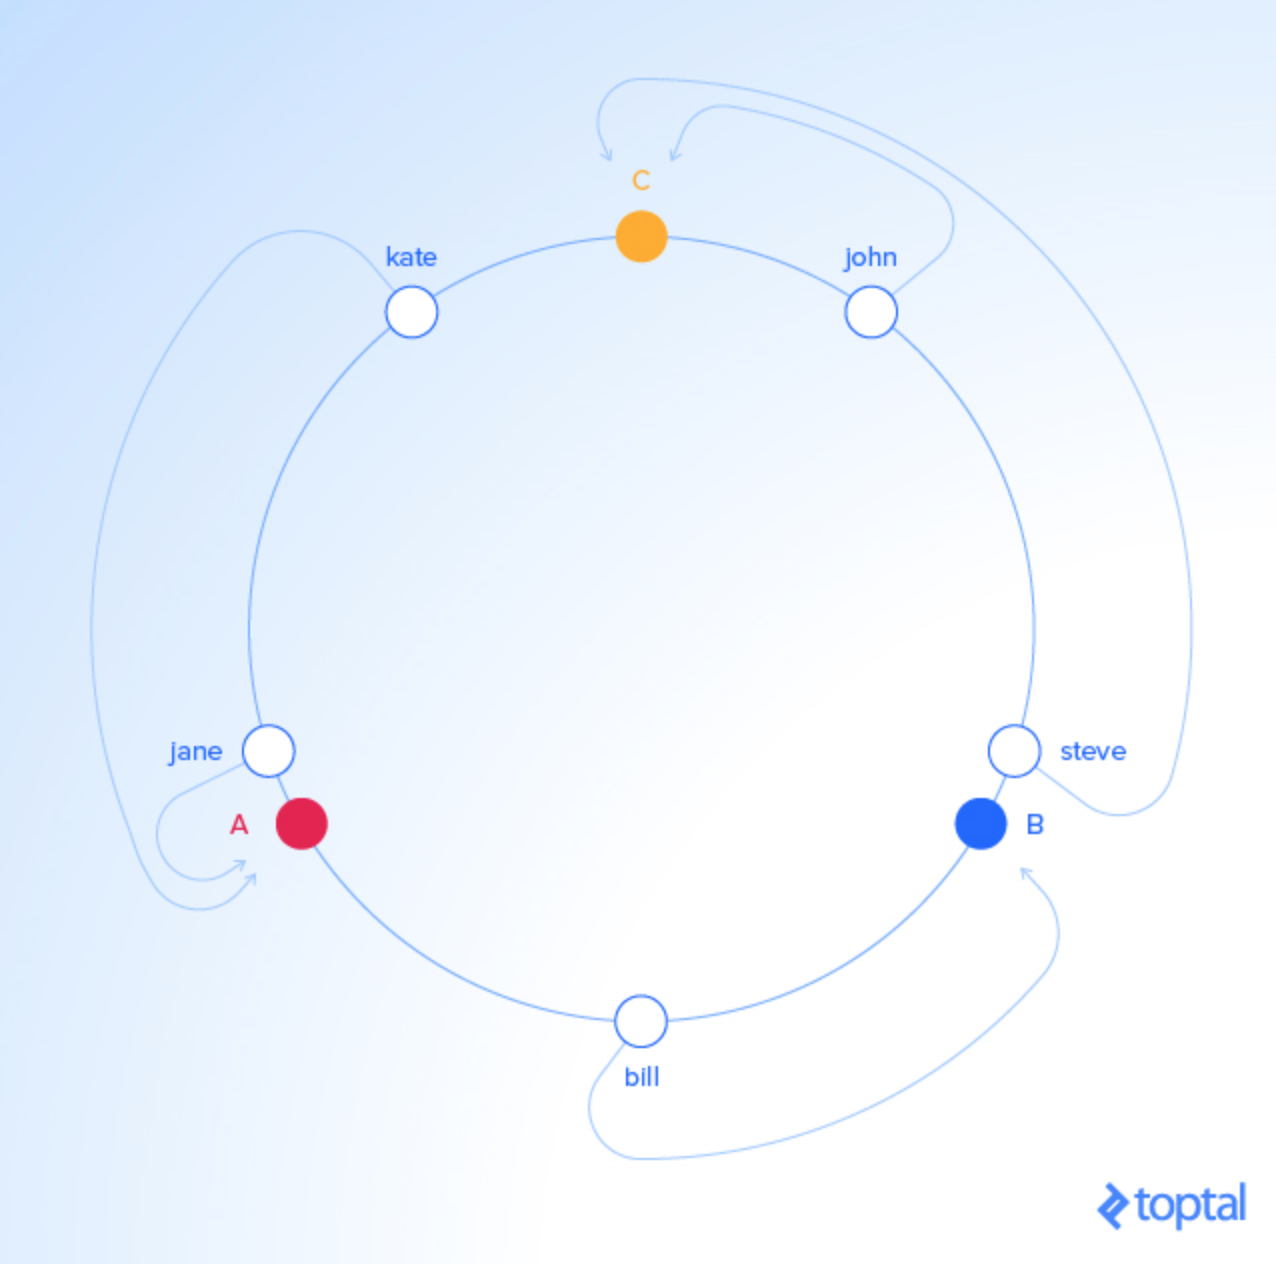
\includegraphics[width=0.55\textwidth]{thesis/figures/hashring.png}  
            \caption{Hash ring example (letters mark the nodes, names mark the objects \cite{ConsistentHashing}}
            \label{ConsistentHashingImage1}
        \end{figure}
        
        To be more consistent and distribute keys evenly among nodes, we can assign nodes not to one but to many places on the hash ring (Figure~\ref{ConsistentHashingImage2}).
        The number of one node keys, known as \textit{weight}, depends on the situation and may be different for each node depending of its capabilities (\textit{heterogeneity}). 
        Thanks to this solution we can easily add or remove nodes to the system and only $\frac{K}{n}$ keys need to be remapped, where $K$ stands for the number of keys and $n$ for the number of nodes.
        

        
        \begin{figure}[ht]
            \centering
                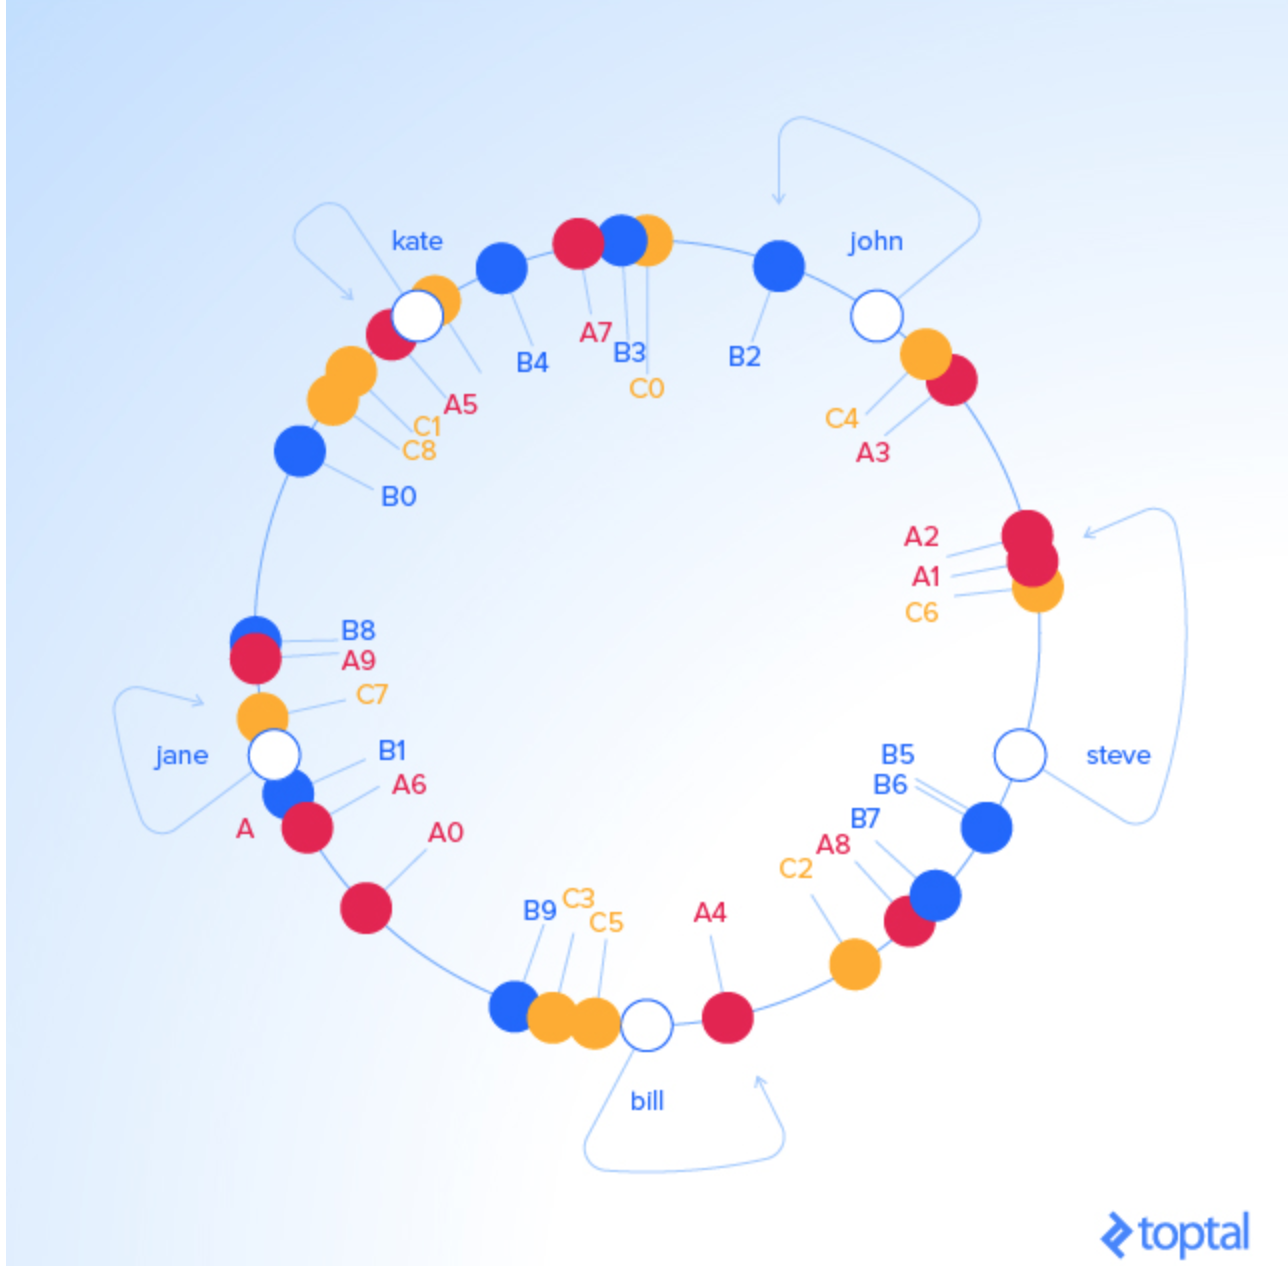
\includegraphics[width=0.55\textwidth]{thesis/figures/vnodes.png}
            \caption{Hash ring example with many node replicas (letters mark the nodes, names mark the objects) \cite{ConsistentHashing}}
            \label{ConsistentHashingImage2}
        \end{figure}
        
    \subsection{Replication} 
        Since distributed systems can fail at any time we need to provide an error prone solution.
        When one of the nodes goes down the whole data it kept is lost.
        This situation is unacceptable in a distributed system.
        Solution to that is keeping replicated data across the nodes.
        For that idea we declare \textit{replication factor} which determines how many times we replicate data.
        With existing \textit{hash ring} every node knows about his neighbours.
        Every node has a copy of his local data in the number of neighbouring nodes depending on that factor.
        Thanks to that when one node becomes unavailable, we can still ask another node about data it kept.
        For that we ask node which is the first replication of unavailable peer.
        If it doesn't respond too then we move to another replication until we get a response.
        
    \subsection{Used libraries}
        For development purpose we wanted to use the best available solution.
        We have looked through different libraries and frameworks and decided to give a try two of them.
        \subsubsection{Seastar}
            \Seastar\cite{Seastar} is an event-driven framework allowing user to write non-blocking, asynchronous code.
            It has support for highly efficient complex server applications on modern multi-core machines.
            Most known use case of \Seastar is ScyllaDB\cite{ScyllaDB} which achieves higher throughputs and lower latencies than her role model Apache Cassandra\cite{Cassandra}.
            \Seastar use two concepts of asynchronous programming which are \textit{futures} and \textit{continuations}.
            Multicore machines have usually a huge overhead for sharing data because of that \Seastar use the share-nothing programming model.
            
            First version of the project used the \Seastar framework but it caused many problems with development.
            Building and configuration process provided by authors is incomplete and needs to be redesigned for project purpose.
            Documentation of \Seastar is missing crucial information and many functions are not described.
            Tests provided with framework were failing for configuration based on Ubuntu 18.04 LTS.
            Project then was migrated to Fedora 27 where configuration process was easier and the tests succeeded.
            \Seastar provides several code samples which we used through reverse engineering to implement a prototype.
            In the process of combining \textit{Persistent Hash Table} with the \Seastar framework a problem occurred. 
            The \Seastar framework performed changes of the \texit{hugepages} \cite{Hugepages} during initialization which made PMDK unable to allocate memory.
            This difficulty was not resolved and the current version of project is not using \Seastar any more.
            
            
        \subsubsection{Boost Asio}
            Asio\cite{Asio} is a C++ library for network programming with a consistent asynchronous model which offers:
            \begin{itemize}
                \item Portability - supports commonly used operating systems.
                \item Scalability - scale to thousands of concurrent connections.
                \item Efficiency - minimise data copying.
                \item BSD sockets
            \end{itemize}